\setcounter{chaptercntr}{1}

\sectionbreak \section*{
  \gostTitleFont
  \redline
  \thechaptercntr .
  АНАЛИЗ ПРЕДМЕТНОЙ ОБЛАСТИ И ПОСТАНОВКА ЗАДАЧИ
}

\titlespace

\subsection*{ 
  \gostTitleFont
  \redline
  \thechaptercntr .\thesubchaptercntr \spc 
  Основные понятия предметной области
} \addtocounter{subchaptercntr}{1}

\subtitlespace

{\gostFont

  \par \redline Объектом исследования и внедрения нейронной сети является пастеризационная установка. Для понимая её технологического процесса, необходимо для начала понять с чем она работает и что она производит, а также какими функциями обладает пастеризационная установка. Поэтому в данной главе мы будем рассматривать пастеризационную установку как некий «серый ящик»: опишем объекты, которые попадают на вход и выходят из пастеризационной установки, а также опишем самые основные процессы, которые происходят с подаваемым на вход объектом. 

  \par \redline И так, основной объект обработки пастеризационной установки является молоко. Поэтому в дальнейшем молоко будет рассматриваться как объект технической обработки. Рассматривая его таким образом, мы понимаем, что оно должно обладать некоторыми показателями, например, состав молока, степень чистоты, кислотность, наличие токсичных и нейтрализующих веществ. При этом молоко обладает ещё и различными свойствами: органолептическими, физико-механическими и биохимическими. И так, разберём лишь те параметры и свойства, которые будут нам в дальнейшем интересны.

  \par \redline Молоко можно разделить на две составляющих: вода и распределённые в этой воде пищевые вещества. К таким веществам относят жиры, белки, углеводы, ферменты, различные минеральные вещества и газы. Помимо этого, в молоке могут находится различные микроорганизмы. И как известно, некоторые из этих микроорганизмов, содержащиеся в молоке, являются опасными или вредными, например, бруцеллеза, ящура, возбудитель кишечной палочки и другие. Но как избавиться от вредных и опасных микроорганизмов?  Для этого используется процесс пастеризации {--} уничтожение различных форм вредных и опасных микроорганизмов в молоке. Но при этом молоко должно сохранить свою биологическую и питательную ценность, а также и своё качество. 

  \par \redline Однако перед тем, как перейти к пастеризации, необходимо определить, какое молоко можно пастеризовать, каким требованиям оно должно соответствовать. Для определения подходящего перед пастеризацией молока существует множество различных показателей и требований. Так, например, пригодное для пастеризации молоко должно быть кислотностью не более 22 °T, а бактериальная обсеменённость молока должна быть один миллион клеток на сантиметр кубический. При этом, молоко не должно быть вспененным. Перед пастеризацией, молоко должно быть также предварительно очищено на фильтрах или на сепараторах-молокоочистителях. Что ж, основные требования перечислены. 

  \par \redline А теперь к самой пастеризации. Основные параметры пастеризации есть температура пастеризации, а также время выдержки, т.е. время нахождения молока в данном процессе. Относительно данных параметров существует выражение, выведенное Г. А. Куком и называемая критерием Пастера. Этот критерий можно рассчитать по формуле (\thechaptercntr .\theformulacntr):

	\formulaspace \par \redline 
    $P=\scaleto{\frac{t}{p}}{20pt}$ 
    \hfill (\thechaptercntr .\theformulacntr) \redline
	\formulaspace \addtocounter{formulacntr}{1}

  \par \redline где $t$ {--} время действия температуры пастеризации, с;

  \par \redline \wherespace $p$ {--} время бактерицидного действия температуры пастеризации, с.  

  \par \redline Что такое бактерицидное действие температуры пастеризации? Это, как раз и есть эффект, в результате которого происходит уничтожение вредных и опасных микроорганизмов. 

  \par \redline Также известна и ещё одна немаловажная зависимость: продолжительность выдержки зависит от температуры пастеризации. Зависимость показана в формуле (\thechaptercntr .\theformulacntr): 
  
  \formulaspace
	\par \redline $\ln{t} = 36.84 - 048T$ \hfill (\thechaptercntr .\theformulacntr) \redline
	\formulaspace \addtocounter{formulacntr}{1}

  \par \redline где $T$ {--} температура пастеризации, $^{\circ}$C.

  \par \redline Завершение процесса пастеризации характеризуется полным уничтожение содержащихся в молоке микроорганизмов. Это можно будет определить благодаря уже известному критерию Пастера, значение которого должно быть не меньше единицы, для того чтобы считать, что процесс пастеризации завершён.  

  \par \redline 	Перед чем, как перейти к описанию пастеризационной установки, следует коротко разобрать ещё одно понятие, с которым мы будем сталкиваться в дальнейшем, а именно гомогенизация. Она представляет собой процесс дробления или уничтожения жировых шариков, образовавшихся в ходе хранения молока. Под воздействием внешних сил можно достичь значительного уменьшения объёма жировых шариков. Процесс гомогенизации позволяет предотвратить самопроизвольное отстаивание жира в молоке на производстве или при его хранении. При этом, гомогенизация даёт возможность сохранить однородную консистенцию молока. Далее рассматривать гомогенизация так подробно, как процесс пастеризации, не имеет смысла, поскольку процесс гомогенизации не является центральным понятием предметной области. 

  \par
}

\subtitlespace

\subsection*{ 
  \gostTitleFont
  \redline
  \thechaptercntr .\thesubchaptercntr \spc
  Результаты обследования пастеризационной установки
} \addtocounter{subchaptercntr}{1}

\subtitlespace

{\gostFont

  \par \redline Пастеризационная установка, она же пастеризационное-охладительная установка, предназначена непосредственно для самой пастеризации, т.е. для уничтожения вредных и опасных микроорганизмов в молоке. Она состоит из множества различных элементов, изучая которые мы также сможем изучить принцип работы пастеризационной установки. Структура пастеризационной установки изображена на рисунке \thechaptercntr .\theimagecntr.

  \par \redline Строго говоря, пастеризационная установка состоит из: 

  \par \redline 1. Балансного танка.
  \par \redline 2. Подающего насоса.
  \par \redline 3. Регулятора потока.
  \par \redline 4. Секции подогрева.
  \par \redline 5. Центробежного очистителя.
  \par \redline 6. Гомогенизатора.
  \par \redline 7. Трубы выдержки.
  \par \redline 8. Вспомогательного насоса.
  \par \redline 9. Системы нагрева горячей входы.
  \par \redline 10. Секции охлаждения.
  \par \redline 11. Возвратного клапана.
  \par \redline 12. Панели управления.

  \begin{sidewaysfigure}
    \centering
    \def\svgwidth{\textwidth}
    \includesvg[scale=0.6]{images/PUS_structure.svg}
    \caption*{\gostFont Рисунок \thechaptercntr .\theimagecntr \spc {--} Визуализация данный 1-ого файла.}
    \label{fig:Data1Visual}
  \end{sidewaysfigure} \addtocounter{imagecntr}{1}

  \par \redline И так, балансный танк является по сути резервуаром с молоком, оборудованным поплавковым входным клапаном, который регулирует расход молока и поддерживает его постоянный уровень в резервуаре. В балансном танке также имеется электрод минимального уровня. Он срабатывает, в том случае, когда уровень молока достигает минимальной точки, тем самым включая клапан распределения потока. Молоко заменяется водой и пастеризатор отключается. 

  \par \redline Подающий насос позволяет обеспечить молоком сам пастеризатор, выкачивая его из балансного танка. 

  \par \redline Для обеспечения устойчивого контроля температуры и постоянного времени выдержки пастеризационной установки используется регулятор потока. Он также необходим для поддержки расхода через пастеризатор на должно уровне.

  \par \redline Молоко, попав в секцию подогрева, должно приобрести некоторую начальную температуру. Это осуществляется с помощью регенерированного тепла некоторого теплоносителя. Для поддержания температуры теплоносителя имеются системы нагрева горячей воды. 

  \par \redline Секцию регенеративного нагрева можно разделить на три секции: секция начального регенеративного подогрева, секция предварительного очищения и секция конечного регенеративного подогрева. Такое разделение используется, поскольку существует необходимость в предварительной обработке молока между входной и выходной температурой молока в секции регенеративного подогрева. Секция начального регенеративного подогрева обычно придаёт молоку температуру около 55-75 $^{\circ}$С. После молоко отправляется в секцию предварительного очищения, представленную центробежным очистителем. После молоко поступает в секцию конечного регенеративного подогрева, где молоко добирает максимальную температуру. 

  \par \redline Эффективность такого нагревания молока регенеративным способом достигает 90-96\%, что отлично сказывается на энергосбережении. Остальную температуру входное молоко добирает за счёт горячей воды, температура которой на 2 или 3 $^{\circ}$С больше температуры пастеризации. Все перечисленные процессы происходят в секции подогрева. Горячая вода имеется благодаря системе нагрева воды.

  \par \redline Нагретое молоко попадает во внешнюю трубу выдержки, где температура проверяется датчиком. Этот датчик беспрерывно контактирует с регулятором температуры на панели управления, а также воздействует на регистрирующий прибор, который сохраняет температуру пастеризации. Тем самым происходит контроль процесса пастеризации.

  \par \redline Как только температура падает ниже минимума, активизируется возвратный клапан, позволяющий пастеризованному молоку попасть в секцию регенеративного охлаждения.
  
  \par \redline Секцию регенеративного охлаждения также можно разделить на две секции: первая секция регенеративного охлаждения и вторая секция регенеративного охлаждения. В первой секции регенеративного охлаждение горячее пастеризованное молоко передаёт свою температуру холодному, предварительно очищенному молоку, находящегося в секции регенеративного конечного подогрева молока. А во второй секции регенеративного охлаждения пастеризованное молоко отдаёт температуру необработанному молоку, находящемуся в секции регенеративного начального подогрева. 

  \par \redline После охлаждённое молоко попадает в секцию охлаждения, которую тоже можно разделить на две секции: первая секция охлаждения и вторая секция охлаждения. В первой секции пастеризованное молоко охлаждается холодной водой, а во второй секции молоко уже охлаждается ледяной водой. 

  \par 
}

\subtitlespace

\subsection*{  
  \gostTitleFont
  \redline
  \thechaptercntr .\thesubchaptercntr \spc
  Введение в прогнозирование, нейронные сети и машинное обучение
} \addtocounter{subchaptercntr}{1}

\subtitlespace

{\gostFont

  \par \redline А сейчас опишем средства, которые будут использоваться для составления прогнозов, а также опишем само понятие прогноза.

  \par \redline Одним из ключевых понятий данной работы является понятие временных рядов. Что же это? Временные ряды {--} это, по сути, некоторая последовательность, каждый элемент из которой состоит из двух или более параметров, а один из них обязательно должен обозначать время. Причём, все эти элементы в последовательности расположены в хронологическом порядке, т.е. в порядке возрастания параметра времени. 

  \par \redline Параметр времени может быть представлен в разных форматах. Выбор формата времени зависит от задачи, удобства использования, длительности, в пределах которой будут собираться данные, а также от требуемой точности. Например, в случае если данные фиксируются раз в день, то хорошо подойдёт отсчёт времени по дням с указанием месяца и года. Если же данные фиксируются в определённые моменты дня, то к вышеописанному стоит прибавить указание часа и минуты фиксации. При необходимости можно указывать и секунды, и миллисекунды. Но что, если нам не особо-то и важно знать, в какой год, месяц или день это происходило, когда нам важно знать, сколько прошло времени от начала того или иного процесса? Тогда, нам скорее подойдёт формат дискретного времени. С помощью этого формата можно узнать длительность процесса в единственной выбранной нами единице измерения времени. Например, если мы сохраняем время в секундах, то 1000-ча секунд сохранит свой формат 1000-чи секунд, время не будет переведено в 16-ать минут и 40-ок секунд. Всё это нам позволяет не привязываться к датам, которые не особо-то и влияют на технологический процесс промышленного оборудования.

  \par \redline Остальные параметры могут уже характеризовать или описывать какой-либо процесс или какие-либо процессы, причём даже не обязательно одного элемента, а даже целой системы элементов. Так, например, когда наш элемент последовательности состоит из двух признаков, а один из которых, как уже известно, время, то второй, конечно же, уже будет обозначать характеристику или состояние изучаемого нами элемента. Но как только у нас появляется три или более признаков, тогда мы уже можем говорить о фиксации характеристик или состояний разных элементов изучаемой системы в один и тот же момент времени или же о фиксации характеристики или состояния одного из множества элементов системы, но с указание этого элемента, например, с помощью идентификационного номера элемента. Как можно убедиться, временные ряды дают весьма гибкую возможность описания процессов или систем относительно времени. 

  \par \redline Технологический процесс пастеризационной установки как раз и представляет собой временной ряд, в котором имеется информация о показаниях различных датчиков в определённые моменты времени. Поэтому, говоря о данных технологического процесса пастеризационной установки, мы будем понимать, что они имеют форму временных рядов.

  \par \redline А что из себя представляет работа с временными рядами? В основном работа делится на две части. Первая часть {--} это понимание структуры временного ряда, его закономерностей, таких как цикличность, тренд, сезонность и так далее, обработка данных временного ряда, визуализация данных, в общем, это всесторонний анализ временного ряда. Если опускать различные математические, статистические и тому подобные подробности, то анализ также может дать нам возможность понять, как начинался процесс, как шёл, развивался и на чём он закончился или остановился на данном моменте времени.  Строго говоря, нейронным сетям, как и исследователям временных рядов, тоже необходимо это понять, чтобы выполнить вторую часть работы, а именно, составление прогноза, что, зачастую, и является основной задачей работы с временным рядом. Да, анализ данных временного ряда технологического процесса делается с целью понять, что будет происходить с этим процессом дальше. Но чем нам так полезна информация о будущем, зачем она нужна? Для этого необходимо понять, что есть прогноз. 

  \par \redline Сам прогноз {--} это некоторая случайная величина, характеризующая вероятность того, что график в будущем пройдёт через определённую точку или некоторую область. Тогда прогнозирование {--} это получение максимально точных прогнозов, или, если говорить в отрыве от понятия прогноза, то это точное предсказание будущего, учитывающее исторические данные об объекте прогнозирования, а также знания о любых будущих событиях, которые могут повлиять на прогнозы. 

  \par \redline Как понять, что прогнозы действительные? Прогнозы являются таковыми, если они отражают подлинные закономерности и взаимосвязи, которые есть в исторических данных, при этом не повторяя прошлые события, которые более не актуальны или уже не повторяются. 

  \par \redline Что необходимо, чтобы составить хороший прогноз на основе временных рядов? Для этого обычно требуется выполнить следующие шаги:

  \par \redline 1. Определить задачу. 
  \par \redline 2. Собрать информацию. 
  \par \redline 3. Произвести предварительный анализ.
  \par \redline 4. Выборать и создать модель прогнозирования.
  \par \redline 5. Использование и оценивание модели прогнозирования. 

  \par \redline Вкратце разберём каждый пункт. При определении задачи необходимо понять, что вообще будет прогнозироваться, как будут использоваться прогнозы, благодаря чему будут получены прогнозы, кому эти прогнозы нужны или для чего. Второй пункт подразумевает непосредственный сбор или получение данных, а также оценка накопленного опыта людей, которые собирают данные и использую прогнозы. Для выполнения третьего пункта необходимо визуализировать данные, составить инфографику, если она необходима, определить взаимосвязь с признаками, закономерности временных рядов, качество данных и так далее, другими словами, провести анализ данных. На четвёртом пункте необходимо либо приобрести и адаптировать готовую модель, либо создать её самостоятельно. Но модель должна учитывать исторические данные, силы взаимосвязи прогнозируемым признаком и любым другим признаком, а также способы использования прогнозов. В заключении проводится тестирование, оценивание, развёртывание и сопровождение модели прогнозирования. 

  \par \redline В дальнейшем на эти пять шагов прогнозирования мы будем ссылаться как на пять этапов составления прогноза.

  \par \redline Теперь поговорим о нейронных сетях и машинном обучении, а также о том, какое место занимает задача прогнозирования в рамках машинного обучения. 

  \par \redline Рассмотрим нейронныю сеть, как некоторую математическую модель и её программную реализацию, которая имитирует работу и взаимосвязи настоящих нейронов.  Рассматривая нейронную сеть как «чёрный ящик», изображённую на рисунке \thechaptercntr .\theimagecntr, мы понимаем, что есть некоторое n входных данных и m преобразованных нейронной сетью выходных данных. В зависимости от назначения сети входные данные могут обозначать исторические данные о процессе, необработанные картинки, зашумлённые чёрно-белые фотографии, текст с ошибками и так далее, а выходными данными могут быть прогнозы, картинки с размеченными на них объектами, восстановленные цветные фотографии, исправленные тексты и так далее. Как можно понять, нейронные сети весьма универсальное средство, которое может решать большой спектр задач. 

  \begin{figure}
    \centering
    \def\svgwidth{\textwidth}
    \includesvg[width=145mm]{images/NNBlackBox.svg}
    \caption*{\gostFont Рисунок \thechaptercntr .\theimagecntr \spc {--} Представление нейронной сети как "чёрный ящик"}
    \label{fig:NNBlackBox}
  \end{figure} \addtocounter{imagecntr}{1}

  \par \redline Нейронная сеть, если её рассматривать уже как «белый ящик», состоит из нейронов. Эти нейроны могут связываться между собой различными способами, например, один нейрон к одному нейрону, один ко многим, иметь обратные связи и так далее. По большей части, то, какие связи имеются между нейронами в сети, определяет, так называемую, архитектуру нейронной сети. Далее нейроны собираются в упорядоченные нейронные слои. Таких слоёв может быть несколько. Тот слой, первый из которых работает с входными данными, называется входным слоем. Слой, который производит расчёт выходных значений, называется выходным слоем. Остальные слои называются скрытыми. Каждый из этих слоёв имеет собственную размерность. На рисунке \thechaptercntr .\theimagecntr \spc нейронные слои изображены как вертикальные последовательности из нейронов, представленных кругами.

  \begin{figure}[H]
    \centering
    \def\svgwidth{\textwidth}
    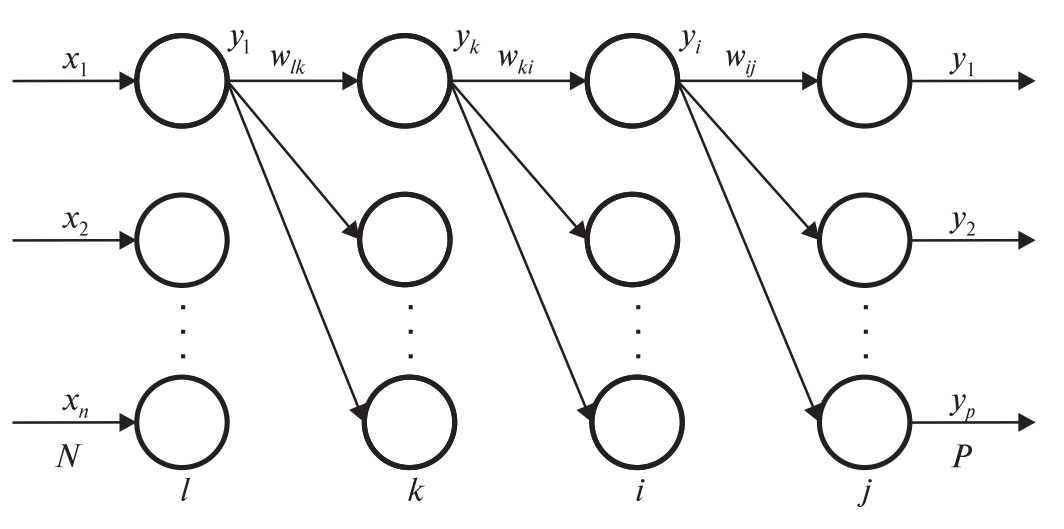
\includegraphics[width=155mm]{images/NNWhiteBox.png}
    \caption*{\gostFont Рисунок \thechaptercntr .\theimagecntr \spc {--} Пример нейронной сети с двумя скрытыми слоями}
    \label{fig:NNWhiteBox}
  \end{figure} \addtocounter{imagecntr}{1}

  \par \redline Слои, как уже было сказано, состоят из нейронов. Каждый нейрон, в свою очередь, состоит из сумматора и активирующей функции. Сумматор необходим для расчёта, так называемой взвешенной суммы, в расчёте которой участвуют как входные значения, так и соответствующие им весовые коэффициенты, а также коэффициенты смещения. Рассчитанная взвешенная сумма преобразуется с помощью некоторой функции активации, образуя тем самым выходные значения нейрона. Данный процесс показан на рисунке \thechaptercntr .\theimagecntr. 

  \begin{figure}[H]
    \centering
    \def\svgwidth{\textwidth}
    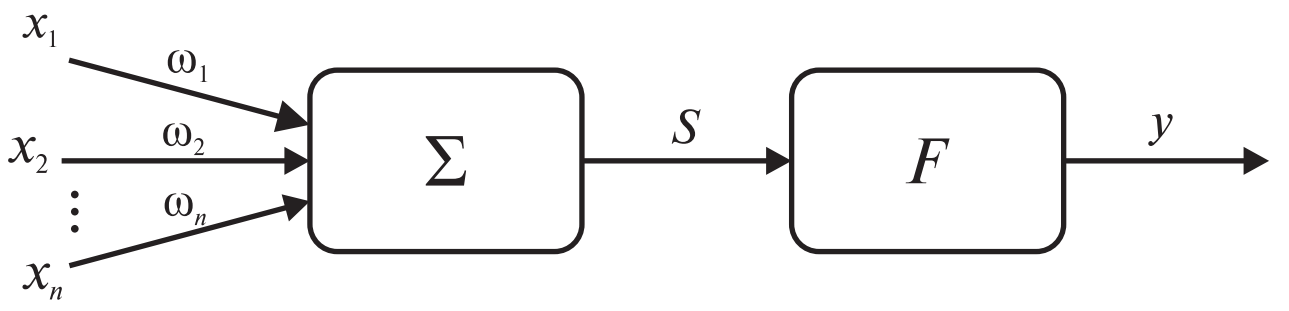
\includegraphics[width=\textwidth]{images/Neuron.png}
    \caption*{\gostFont Рисунок \thechaptercntr .\theimagecntr \spc {--} структура нейронного элемента}
    \label{fig:Neuron}
  \end{figure} \addtocounter{imagecntr}{1}

  \par \redline Для ясности, нижу будет представлен поэтапный пример расчёта нейронного элемента.

  \par \redline В начале, как уже было ранее сказано, рассчитывается взвешенная сумма с помощью формулы (\thechaptercntr .\theformulacntr):

	\formulaspace
	\par \redline $S = w_1 \cdot x_1 + w_2 \cdot x_2 + \dots + w_n \cdot x_n + b$ \hfill (\thechaptercntr .\theformulacntr) \redline
	\formulaspace \addtocounter{formulacntr}{1}

  \begin{tabular}{p{0,875cm}p{0,3cm}p{15,175cm}}
		& где  & $S$ {--} взвешенная сумма; \\
		& 	   & $x_n$ {--} n-тое входное значение; \\
    & 	   & $w_n$ {--} n-тое значение весового коэффициента; \\
    & 	   & $b$ {--} коэффициент смещения. \\
  \end{tabular}

  \par \redline Выходные значения нейронного элемента рассчитываются по формуле (\thechaptercntr .\theformulacntr):

	\formulaspace
	\par \redline $y = F \left(S\right)$ \hfill (\thechaptercntr .\theformulacntr) \redline
	\formulaspace \addtocounter{formulacntr}{1}

  \begin{tabular}{p{0,875cm}p{0,3cm}p{15,175cm}}
		& где  & $F({...})$ {--} функция активации; \\
		& 	   & $y$ {--} выходное значение нейронного элемента. \\
  \end{tabular}

  \par \redline И так, теперь перейдём к машинному обучению – набор алгоритмов, благодаря которым осуществляется обучение нейронной сети. А её обучение можно ещё определить, как подбор или поиск таких значений весов и смещений или порогов каждого нейрона, чтобы нейронная сеть выдавала необходимые результаты. 

  \par \redline Теперь давайте определим, как связана задача прогнозирования и машинное обучение, чтобы обучить нейронную сеть предсказывать будущее. Для понимания этого, нужно иметь ввиду, что машинное обучение делится на четыре направления: обучение с учителем, обучение без учителя и обучение с подкреплением. 

  \par \redline Однако, для начала необходимо разъяснить несколько понятий, которые используются в лексике машинного обучения. Первое из таких понятий это понятие признака – некоторое измерение или параметр, определяющий характеристику или состояние чего-либо. Следующее понятие есть метка – по сути то, чему должен соответствовать признак.  И в конце концов, пример – это то, что подаётся на вход нейронной сети. Существуют помеченные и непомеченные примеры. Помеченные примеры — это такие примеры, которые состоят из пар признаков и меток, т.е. $\left\{\left(x_{1}, y_{1}\right), \left(x_{2}, y_{2}\right), \dots, \left(x_{n}, y_{n}\right)\right\}$, или такие примеры, в которых каждому вектору или каждой последовательности признаков соответствует вектор или последовательность меток $\left\{\left(X_{1}, Y_{1}\right), \left(X_{2}, Y_{2}\right), \dots, \left(X_{n}, Y_{n}\right)\right\}$. Непомеченные примеры, это по факту просто признаки, т.е. $\left\{x_{1}, x_{2}, \dots, x_{n}\right\}$. 

  \par \redline И так, говоря об отличии между обучением с учителем и обучением без учителя, можно сказать, что обучение с учителем использует помеченные примеры, а обучение без учителя использует непомеченные примеры. 

  \par \redline Теперь пару слов про обучение с подкреплением {--} раздел машинного обучения, в котором рассматривается ситуация, когда машина <<обитает>> в некоторой окружающей среде и способна воспринимать состояние этой среды как вектор признаков. Это чем-то напоминает обучение без учителя, поскольку нейронной сети также подаётся вектор признаков $\left\{x_{1}, x_{2}, \dots, x_{n}\right\}$, но в нейронную сеть также поступает сигналы подкрепления из некоторой внешней среды, в которой находится сеть.

  \par \redline	Рассмотрим задачу прогнозирования и определим, какими примерами мы оперируем, чтобы выбрать подходящую модель обучения модели нейронной сети. И так, для прогнозирования используются исторические данные, а данных из будущего у нас нет. В таком случае, как бы мы не рассчитывали будущее с помощью нейронных сетей на основе исторических данных без проверки с тем, что должно получиться, мы не достигнем никаких результатов. Нам необходимы некоторые эталоны, с которыми мы могли сравнивать полученные результаты сети. Откуда их брать? Чтобы их получить мы разделим исторические данные на примеры и соответствующие им эталоны, т.е. метки. Таким образом для обучения сети мы получим помеченные данные, в которых каждому вектору признаков, взятого из исторических данных, будет соответствовать вектор меток, взятых из тех же исторических данных, взятых сразу после последнего значения вектора признаков из общей последовательности исторических данных. Тем самым, мы говорим, что наша задача прогнозирования может быть решена с помощью нейронных сетей и машинного обучения.

  \par \redline Раз мы определились, что мы будем использовать машинное обучения для решения задачи прогнозирования, стоит пару слов сказать о инженерии машинного обучения, которая поможет достичь нам необходимых результатов. Рассмотрим этапы инженерии машинного обучения, которые определят последовательность дальнейшей работы:

  \par \redline 1. Определение задачи и цели. 
  \par \redline 2. Сбор и подготовка данных. 
  \par \redline 3. Конструирование признаков.
  \par \redline 4. Обучение модели.
  \par \redline 5. Оценка модели.
  \par \redline 6. Развёртывание модели.
  \par \redline 7. Обслуживание запросов к модели.
  \par \redline 8. Мониторинг модели.
  \par \redline 9. Сопровождение модели. 

  \par \redline Первый, второй и третий этапы инженерии машинного обучения схожи с первыми тремя этапами составления прогноза. На этапе обучения модели производится непосредственно само обучение сети, по правилам, в соответствии с типом обучения. На пятом этапе проводится всесторонняя оценка модели, а также настройка некоторых её элементов. Именно на этом этапе делается вывод о готовности модели нейронной сети выполнять поставленные задачи. После наступает этап развёртывания нейронной сети, в ходе которого модель нейронной сети попадает в целевую среду для выполнения поставленных перед ней задач. На этапе обслуживания запросов необходимо убедиться в том, что на входы нейронной сети будут попадать данные такого формата, который будет понятен модели, и что сеть выдаёт необходимые результаты. Другими словами, это вопросы снабжения модели сети всем необходимым для её функционирования. Далее идёт этап мониторинга нейронной сети и её сопровождения. По факту это этапы использования сети по назначению.    

  \par \redline Изучив этапы инженерии машинного обучения, становится понятно, что необходимо сделать, чтобы была создана модель нейронной сети, способная давать приемлемые результаты. Поэтому дальнейшая работа будет развиваться относительно этапов инженерии машинного обучения.

  \par \redline И так, порядок работы определён, поэтому в следующей главе будет разобрано, какие требование предъявляются к самой модели для прогнозирования, после будут определены цели и задачи прогнозирования, выполнив тем самым первые этапы инженерии машинного обучения и построения прогноза.

  \par
}

\subtitlespace

\subsection*{
  \gostTitleFont
  \redline
  \thechaptercntr .\thesubchaptercntr \spc
  Требования к модулю прогнозирования и постановка задачи
} \addtocounter{subchaptercntr}{1}

\subtitlespace

{\gostFont

  \par \redline Модуль прогнозирования должен выполнять прогноз технологического процесса пастеризационной установки. Для этого ему необходимо получать данные технологического процесса пастеризационной установки с помощью программируемого микроконтроллера, использующего платформу PLCnext Technology. По этой причине, программа должна быть написана на низкоуровневом языке программирования, а именно на C++, который поддерживается данным микроконтроллером. 

  \par \redline Поскольку процесс пастеризации происходит непрерывно, то программа должна работать в режиме реального времени и своевременно снабжать необходимой информацией о прогнозах поведения пастеризационной установки. 

  \par \redline Программа должно быть устойчива к различным сбоям и авариям, а также не создавать их сама. 

  \par \redline Должна быть предоставлена возможность вносить некоторые настройки в модуль прогнозирования для корректировки работы модели нейронной сети. 

  \par \redline Для постановки задачи, необходимо понимать, что сама программа, которая будет в дальнейшем использоваться для прогнозирования данных временных рядов технологического процесса пастеризационной установки, будет использовать нейросетевое решение задачи прогнозирования. Для обучения модели нейронной сети применяются алгоритмы машинного обучения, от которых зависит качество модели прогнозирования. Оттого данная работа в основном и будет развиваться по этапам инженерии машинного обучения, и потому данная работа будет являться проектом машинного обучения. 

  \par \redline Задачей для проекта машинного обучения будет является разработка модуля прогнозирования данных временных рядов пастеризационной установки с целью прогноза поведения пастеризационной установки, планирования производства, а также выявления аномального поведения, возможных сбоев и выбросов пастеризационной установки. 

  \par \redline Для выполнения поставленной задачи необходимо изучать данные технологического процесса, а также провести их анализ и обработку. Далее необходимо выбрать подходящую архитектуру нейронной сети, построить и обучить модель сети, после чего организовать эффективное обучение сети, используя алгоритмы машинного обучения.  Написать код нейронной сети необходимо на низкоуровневом языке программирования для дальнейшего развёртывания на программируемом контроллере, взаимодействующим с пастеризационной установкой. 

  \par \redline Также необходимо произвести тестирование и оценку качества полученной модели. После чего непосредственно выполнить процесс развёртывания нейронной сети.  

  \par 
}

\setcounter{subchaptercntr}{1}
\setcounter{formulacntr}{1}
\setcounter{imagecntr}{1}
